\documentclass[tikz,border=10pt]{standalone}
\begin{document}
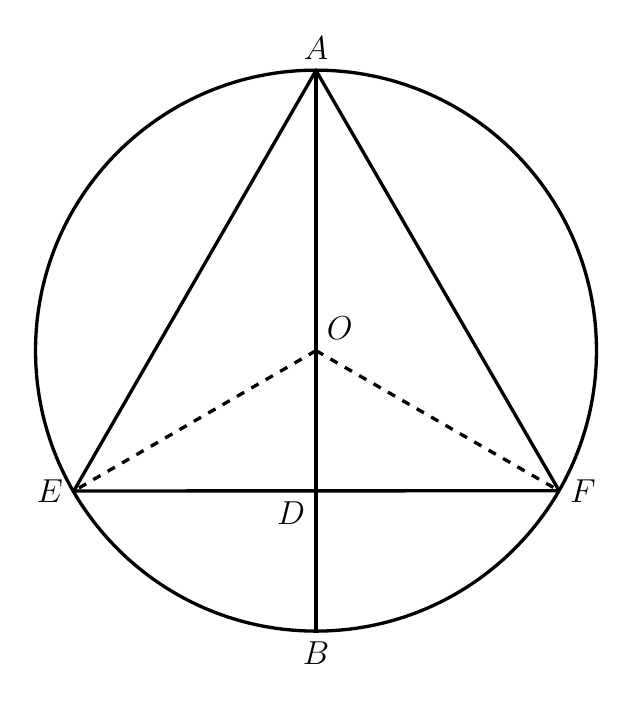
\begin{tikzpicture}[line width=1.2pt, line join=round]
% Named coordinates; origin at O, 1 unit = 1 cm (s = 0.015094 px per unit from STYLE METRICS)
\coordinate (O) at (0,0);
\coordinate (A) at (0,3.558);
\coordinate (B) at (0,-3.560);
\coordinate (D) at (0,-1.782);
\coordinate (E) at (-3.076,-1.782);
\coordinate (F) at (3.088,-1.780);

% Circle centred at O
\draw (O) circle[radius=3.562];

% Solid vertical diameter AB (passes through D)
\draw (A) -- (B);

% Solid horizontal chord EF at y = D
\draw (E) -- (F);

% Solid segments AE and AF
\draw (A) -- (E);
\draw (A) -- (F);

% Dashed radii OE and OF
\draw[dashed] (O) -- (E);
\draw[dashed] (O) -- (F);

% Point labels (math mode, label font from metrics)
\node[font=\fontsize{12}{14.4}\selectfont, above] at (A) {$A$};
\node[font=\fontsize{12}{14.4}\selectfont, below] at (B) {$B$};
\node[font=\fontsize{12}{14.4}\selectfont, below left] at (D) {$D$};
\node[font=\fontsize{12}{14.4}\selectfont, left] at (E) {$E$};
\node[font=\fontsize{12}{14.4}\selectfont, right] at (F) {$F$};
\node[font=\fontsize{12}{14.4}\selectfont, above right] at (O) {$O$};
\end{tikzpicture}
\end{document}